\documentclass[11pt,a4paper]{article}
\usepackage[T1]{fontenc}
\usepackage{lmodern}
\usepackage{microtype}
\usepackage[margin=2.6cm]{geometry}
\usepackage{booktabs}
\usepackage{graphicx}
\usepackage{caption}
\usepackage[hidelinks]{hyperref}
\setlength{\parindent}{0pt}
\setlength{\parskip}{0.6em}

\title{Forecasting return distributions after SEC filings}
\author{Hermes Reisner}
\date{Findings, November 2026}

\begin{document}
\maketitle

Built and tested on a real dataset of 11,569 company filings, with the last 3,329 kept aside for the final test. For every filing, it forecasts how much the company's stock can move. The model is a small Transformer that tries an idea from the very frontier of open source prediction models: it first learns on simulated companies and only then on real filings.

\section*{What I tested}

The dataset is 11,569 quarterly and annual reports of 305 US industrial companies from 2010 to 2026, all taken from the SEC's \href{https://www.sec.gov/search-filings}{EDGAR} database. The model doesn't try to predict a long-term development but the risk right after a filing, which is how far the stock can move against the industrial sector fund (XLI) over the next 5 and 20 trading days. The clock starts at the first market open at least 30 minutes after the SEC accepted the report as this is when people can start to act on it.

I first trained the model on simulated companies with invented reporting habits and then on the real filings before 2022, and kept 2022 for validation. Before the final test, I wrote the rules down and saved a checksum of them, and the code refuses to compute any result if that file changes. The model had four opponents: a forecast that only knows how jumpy the stock has been, a linear model, boosted trees, and the same network without the simulator.

\section*{What came out}

\begin{table}[ht]
\centering
\small
\begin{tabular}{lrc}
\toprule
network against & change in loss [95\,\% interval] & verdict \\
\midrule
volatility forecast & $-3.36\,\%$ [$-4.14$, $-2.56$] & supported \\
linear model & $-2.06\,\%$ [$-2.94$, $-1.01$] & supported \\
boosted trees & $-1.91\,\%$ [$-2.65$, $-1.05$] & supported \\
same network without the simulator & $-0.18\,\%$ [$-0.58$, $+0.22$] & not supported \\
\bottomrule
\end{tabular}
\end{table}

In the final test (3,329 filings from 2023 to 2026), the network's loss was 3.4\,\% lower than the volatility forecast, 2.1\,\% lower than the linear model and 1.9\,\% lower than the boosted trees. That held in all three runs and even on 867 filings from companies it had never seen. The simulator was not the reason. The same network trained only on real filings was 0.2\,\% behind, which is inside the noise.

\begin{figure}[ht]
\centering
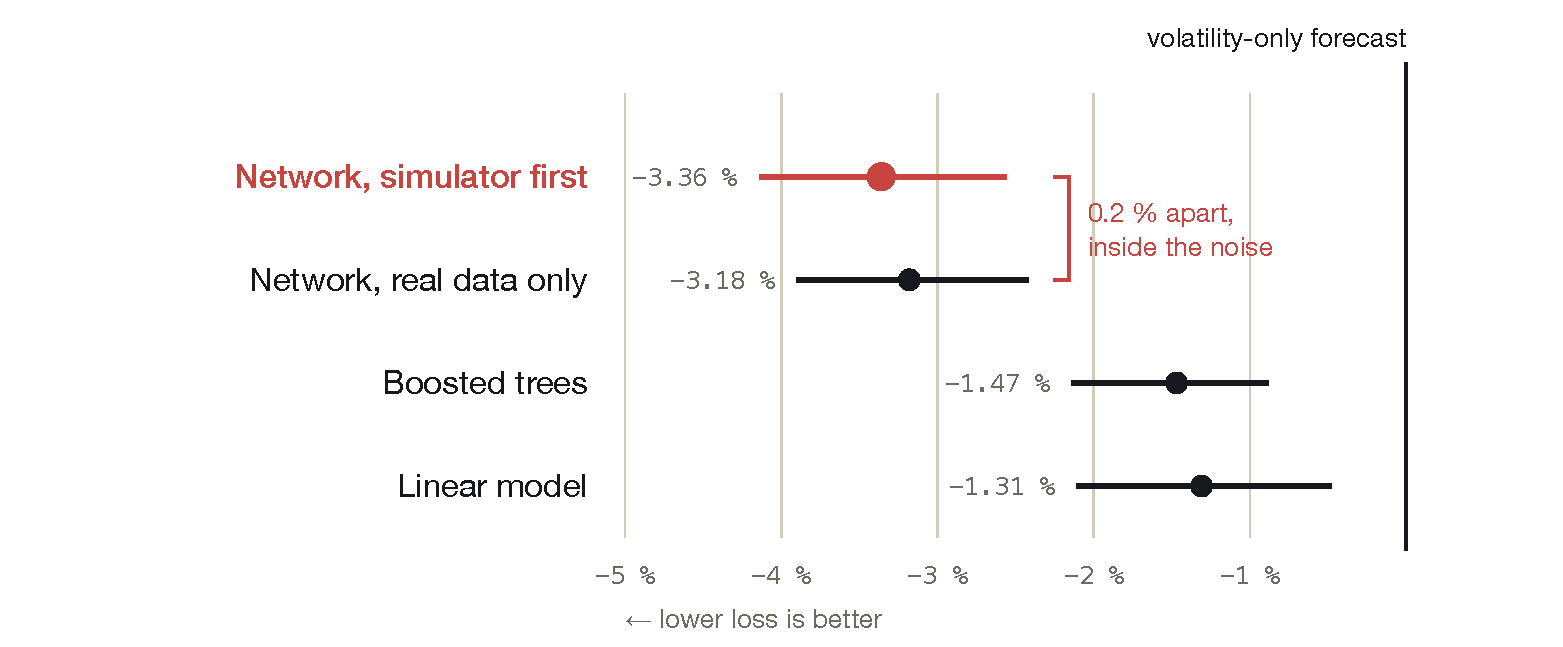
\includegraphics[width=0.8\linewidth]{figures/forest.pdf}
\caption*{\small Change in loss against the volatility forecast on 2023 to 2026, with 95\,\% intervals.}
\end{figure}

What the network doesn't know is which way a stock goes. The network, the linear model and the trees were each right about 50\,\% of the time. The volatility forecast got 54.4\,\%, but only because its middle is always slightly below zero, which is the same as always guessing ``down''. I checked this afterwards, so it was not part of the written rules. So the whole edge is in how wide the range of outcomes is. It also didn't hold every year: in 2019 the network was 3.6\,\% better than the volatility forecast, and in 2020 it was 1.7\,\% worse. And that volatility forecast is a simple one. The trees did as well without the filings as with them, and a version of the network with a memory for corrections did nothing, not even in simulation.

\begin{figure}[ht]
\centering
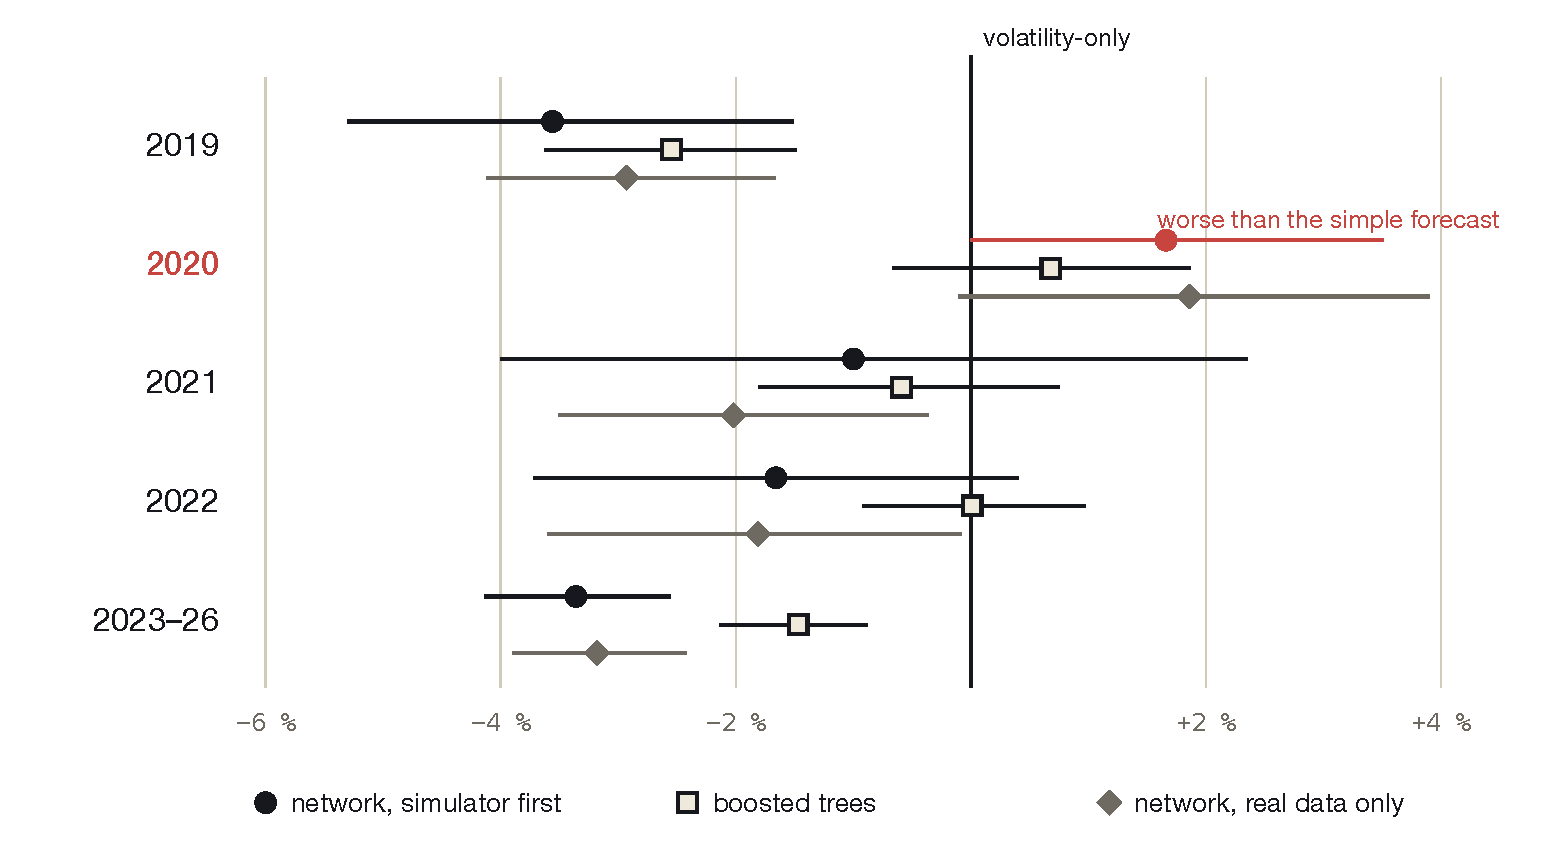
\includegraphics[width=0.8\linewidth]{figures/byyear.pdf}
\caption*{\small Each test period on its own, against the volatility forecast.}
\end{figure}

\begin{figure}[ht]
\centering
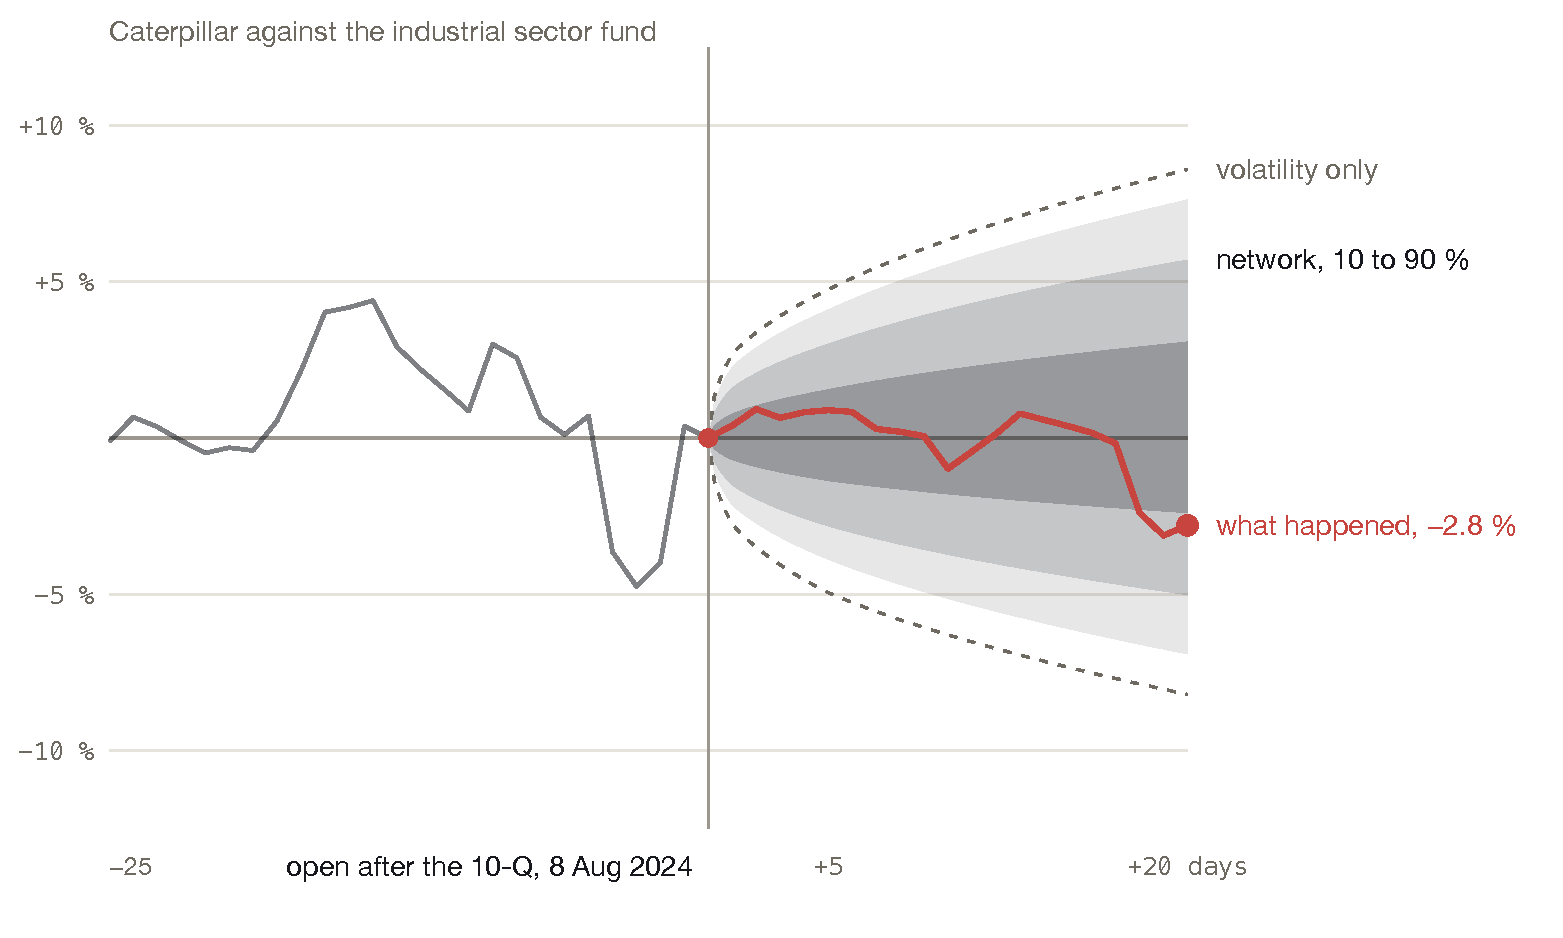
\includegraphics[width=0.8\linewidth]{figures/fan.pdf}
\caption*{\small One forecast: Caterpillar after its 10-Q of 7 August 2024. Shaded: the network\textquotesingle s 5--95, 10--90 and 25--75\,\% ranges. Dashed: the volatility forecast. Red: what happened.}
\end{figure}

\section*{The data}

The numbers come from the SEC's XBRL data with every version kept, so the model only sees a value the way it was known on that day. Getting the data right took more time than the model. The SEC's bulk download says its acceptance times are in UTC. For about two thirds of the 46,854 filings I needed, they are not: 17.1\,\% are New York time with a UTC label and 49.3\,\% are shifted twice. The New York error follows the company, so either all of its filings have it or none do. Therefore all times come from the SEC's XBRL archive and the filing pages instead.

A sample of 120 random records was checked against the original filings. Revenue matched in 30 of 30 cases, inventory in 30 of 30, backlog only in 15 of 20. Orders and guidance, the reason I picked industrial companies, don't exist as clean data at all. Of the 77 values I could trace, 61 were already in the earnings press release, so the filing is often late news. An AI agent recorded the verdicts from the source snippets, and every row links to its filing so it can be checked again. The prices come from Yahoo, which only has companies that are still listed, so 9,666 of 26,949 possible filings were lost.

\section*{How the model works}

The network is a pre-norm Transformer encoder with 6 layers, width 256, 8 attention heads and no dropout, 5,140,487 parameters in total. It reads three kinds of tokens. A fact token is one of up to 128 revenue or inventory records, which a linear layer and a GRU cell build from 10 numbers: the year-over-year growth, which metric it is, its version, whether it is a revision, how old the period and the record are, and how late it was reported. A market token is one of 96 trading days and holds the excess return against XLI, its absolute value, the position in the window, and how many earnings releases and filings came out that day. At the end, three learned query tokens, one per horizon (1, 5 and 20 sessions), collect the answer.

Each query outputs seven quantiles (5, 10, 25, 50, 75, 90 and 95\,\%). They can't cross, because the model only predicts the median and positive steps outwards (a softplus, summed up), which are in units per square root of a session and then get scaled by $\sqrt{h}$. The loss is the pinball loss over the seven quantiles, divided by $\sqrt{h}$, so the 20-day horizon doesn't dominate.

Pretraining ran on 300 million tokens of simulated companies (20,650 steps, batch 64, AdamW at $5\cdot10^{-4}$, bf16 on an RX 9060 XT). Every simulated company has an economic process, a disclosure process that decides when numbers come out, how late and how often they get revised, and a market that reacts to it. In 40\,\% of these worlds the filings say nothing about future returns, so the model learns not to invent a signal where there is none. Fine-tuning on the real filings used AdamW at $2\cdot10^{-4}$ with cosine decay, at most 15 epochs and early stopping on 2022.

The volatility forecast scales the last 20 days' volatility by $\sqrt{h}$ and takes its quantiles from the training data. The linear model is one quantile regression per quantile and horizon, and the trees are gradient-boosted quantile models on hand-built features with the same information. Between training and test there is a gap of 20\,+\,5 sessions, so no label can leak, and the confidence intervals come from 2,000 bootstrap resamples of whole weeks.

\section*{What I would do next}

The volatility forecast only uses the last 20 days, so a GARCH-type model on the same window is the obvious next opponent. The decision should also move to the earnings press release, because most of the numbers are already public there. And testing on companies that disappeared needs a price source with delisted stocks, which the free ones don't have.

AI agents did most of the coding and running: Codex for the first setup, Claude for the pipeline and the analysis, and Gemini to supervise the long runs.

The code is at \url{https://github.com/HerRei/sec-filing-forecasts}.

\end{document}
